\section{Scenarios}\label{sec:scenarios}
In the following subsection, we discuss a selection of scenario flows. This selection is based on the priority of the use cases or on interesting behaviour of the system they showcase.

\subsection{Av2 - PDSDBReplica back on-line}
Figure \ref{fig:seq_av2online} describes what happens when a previously failed replica comes back on-line. When the failed replica responds to a ping from the \ttt{PDSReplicationManager}, the \ttt{PDSReplicationManager} asks another replica for all documents that have been stored since failure was detected. Upon reception of these documents, they are all stored in the previously off-line replica. This way, that replica is brought back up to speed.

\begin{figure}[!htp]
    \centering
    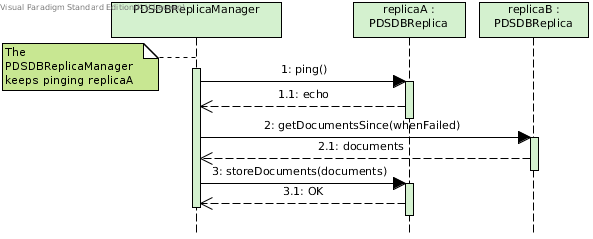
\includegraphics[width=0.7\textwidth]{figures/Av2 - PDSDBReplica back on-line.png}
    %\missingfigure[figwidth=0.8\textwidth]{Sequence diagram scenario 1}
    \caption{The system behavior for recovery from \ttt{PDSDBReplica} failure.
        }\label{fig:seq_av2online}
\end{figure}

\subsection{Av2 - PDSDBReplica fails}
Figure \ref{fig:seq_av2fail} describes how failure of a \ttt{PDSReplica} is detected and which actions are taken. If the \ttt{PDSReplicationManager} issues a query to a \ttt{PDSDBReplica} and it does not respond within four seconds, the \ttt{PDSDBReplica} is pinged. If that ping times out, the \ttt{PDSDBReplica} is perceived as having failed and a notification to the eDocs administrators is issued through the \ttt{CommunicationSubsystem}.

\begin{figure}[!htp]
    \centering
    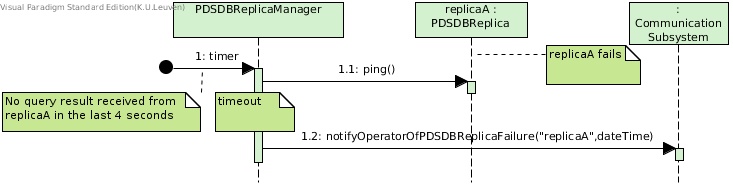
\includegraphics[width=0.8\textwidth]{figures/Av2 - PDSDBReplica fails.png}
    %\missingfigure[figwidth=0.8\textwidth]{Sequence diagram scenario 1}
    \caption{The system behavior for detection of \ttt{PDSDBReplica failure}.
        }\label{fig:seq_av2fail}
\end{figure}

\subsection{UC1 - Login}
Figure \ref{fig:seq_uc1} shows the steps taken to log in a user. Logging in consists of trying to create a session using the credentials supplied by the user. The first concern is verifying the user's credentials, which is the responsibility of the \ttt{AuthenticationManager}. Depending on the type of login request, the login details matching the supplied username are fetched from either the \ttt{RegisteredRecipientDatabase}, \ttt{COAdminDatabase} or \ttt{eDocsAdminDatabase}. After the login details have been received, the supplied credentials and the login details are compared. If successful, the \ttt{AuthenticationManager} returns a login token, upon which the session can be created. If unsuccessful, an AuthException is thrown and it is indicated to the user he supplied invalid credentials.

\begin{figure}[!htp]
    \centering
    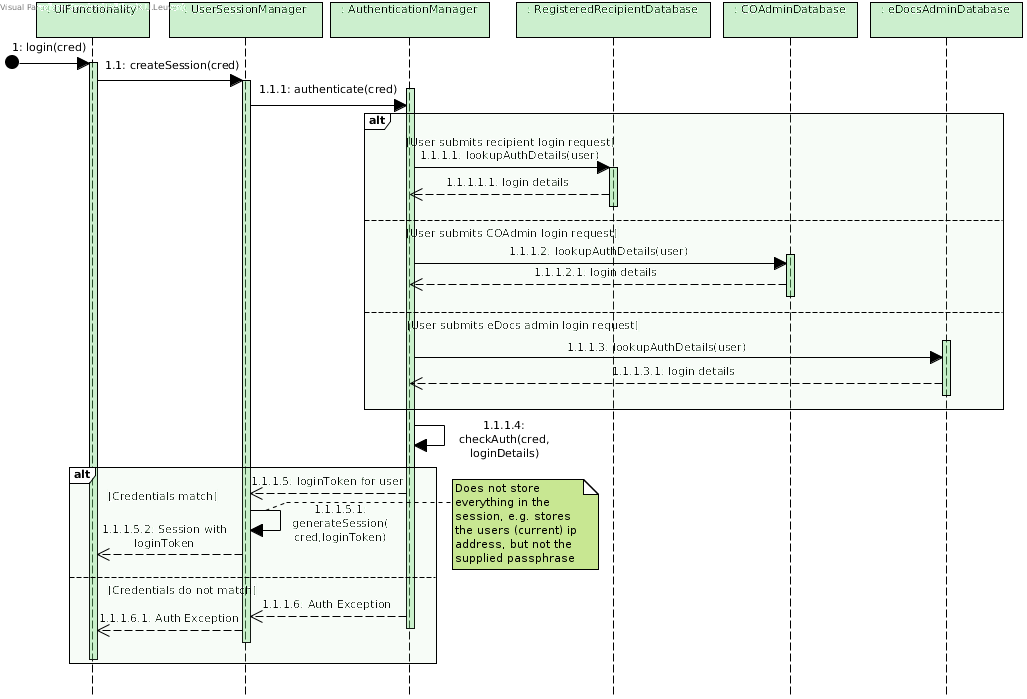
\includegraphics[width=\textwidth]{figures/UC1 - Login.png}
    %\missingfigure[figwidth=0.8\textwidth]{Sequence diagram scenario 1}
    \caption{The system behavior for Use Case 1.
        }\label{fig:seq_uc1}
\end{figure}

\subsection{UC3 - Initiate document processing}\todo{fix sequence diagram: submitJobs}
Figure \ref{fig:seq_uc3} shows the steps taken to submit raw data, with some minor details omitted for brevity. First, the data submitter sends details about the batch they plan to submit. These batch details are first verified by the \ttt{RawDataVerifier} and an exception is thrown when something is out of order (refer to section \ref{sec:rawdataverifier} for details about when the exception is thrown). When the batch details have been successfully verified, the submitter uploads the batch. Now, all individual entries are verified. If any individual entries fail verification, an exception is thrown and it is indicated which entries failed and why (again, refer to section \ref{sec:rawdataverifier} as to what exactly is verified). All entries that passed verification are now supplied to the \ttt{JobGenerator}, where \ttt{Job} objects are generated and finally passed to the \ttt{JobSubmitter}, which stores them. The \ttt{Job}s are also passed to the \ttt{Scheduler} so that document generation may begin. 

\begin{figure}[!htp]
    \centering
    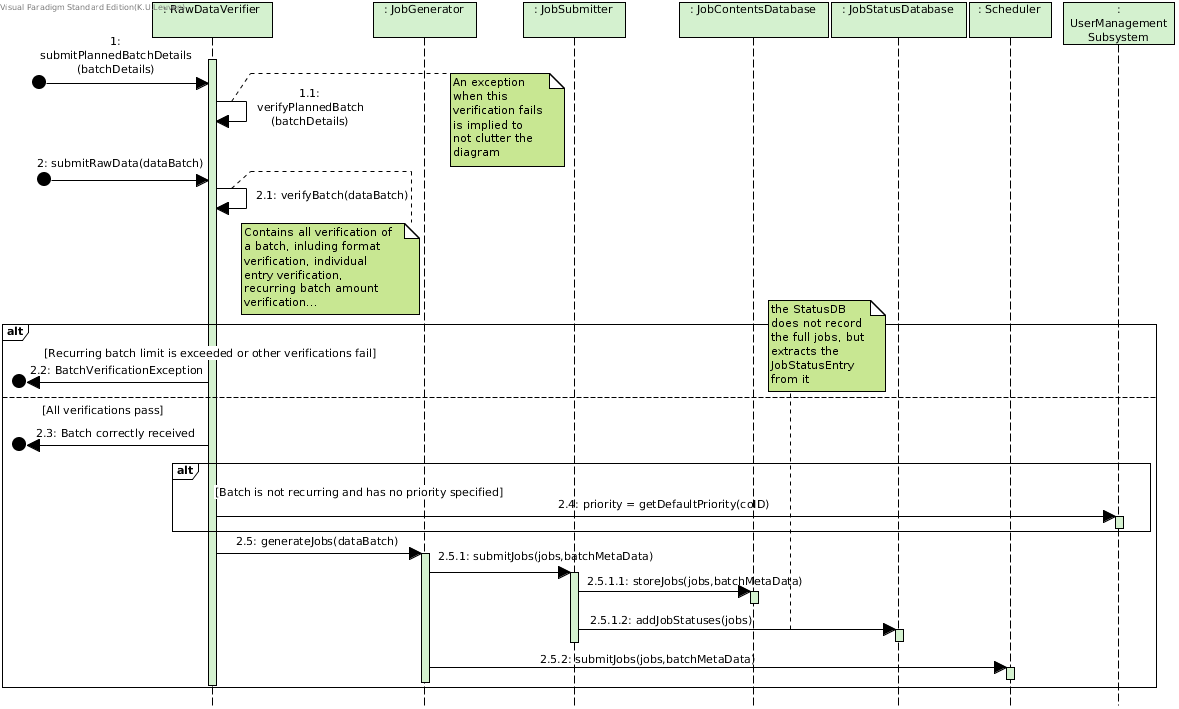
\includegraphics[width=\textwidth]{figures/UC3 - Initiate document processing.png}
    %\missingfigure[figwidth=0.8\textwidth]{Sequence diagram scenario 1}
    \caption{The system behavior for Use Case 3.
        }\label{fig:seq_uc3}
\end{figure}

\subsection{UC4/5 - Process Jobs}
Figures \ref{fig:seq_uc45_1} and \ref{fig:seq_uc45_2} show how documents are generated. One way or the other, the \ttt{Generator} receives a new batch to work on. It then asks the \ttt{Completer} to fetch the raw data and meta-data, which asks the \ttt{JobStorageSystem} in turn. We assume here that it concerns an invoice, therefore the key is needed. The \ttt{KeyCache} is asked for it, which asks the \ttt{UserManagementSubsystem}, if necessary. Next, the \ttt{Completer} asks the \ttt{TemplateCache} for the template. The \ttt{UserManagementSubsytem}

\begin{figure}[!htp]
    \centering
    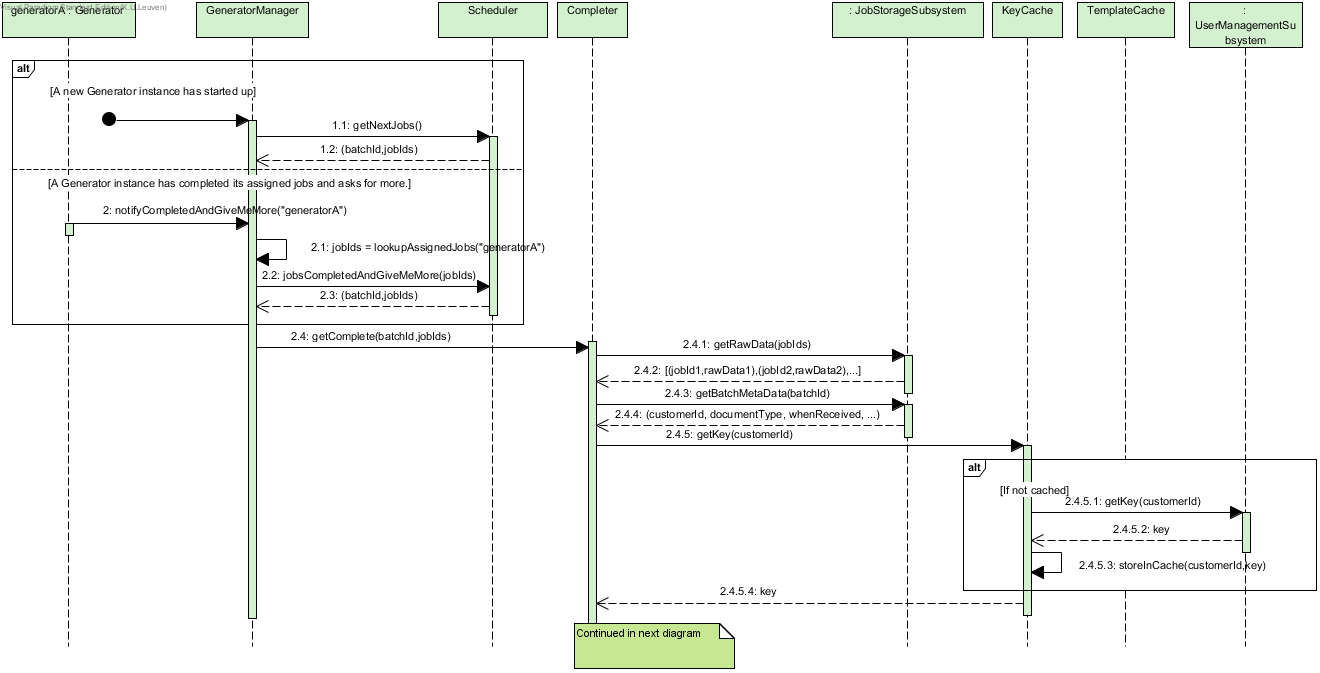
\includegraphics[width=\textwidth]{figures/UC4_5 - ProcessJobs1.png}
    %\missingfigure[figwidth=0.8\textwidth]{Sequence diagram scenario 1}
    \caption{The system behavior for Use Cases 4 and 5.
        }\label{fig:seq_uc45_1}
\end{figure}

\begin{figure}[!htp]
    \centering
    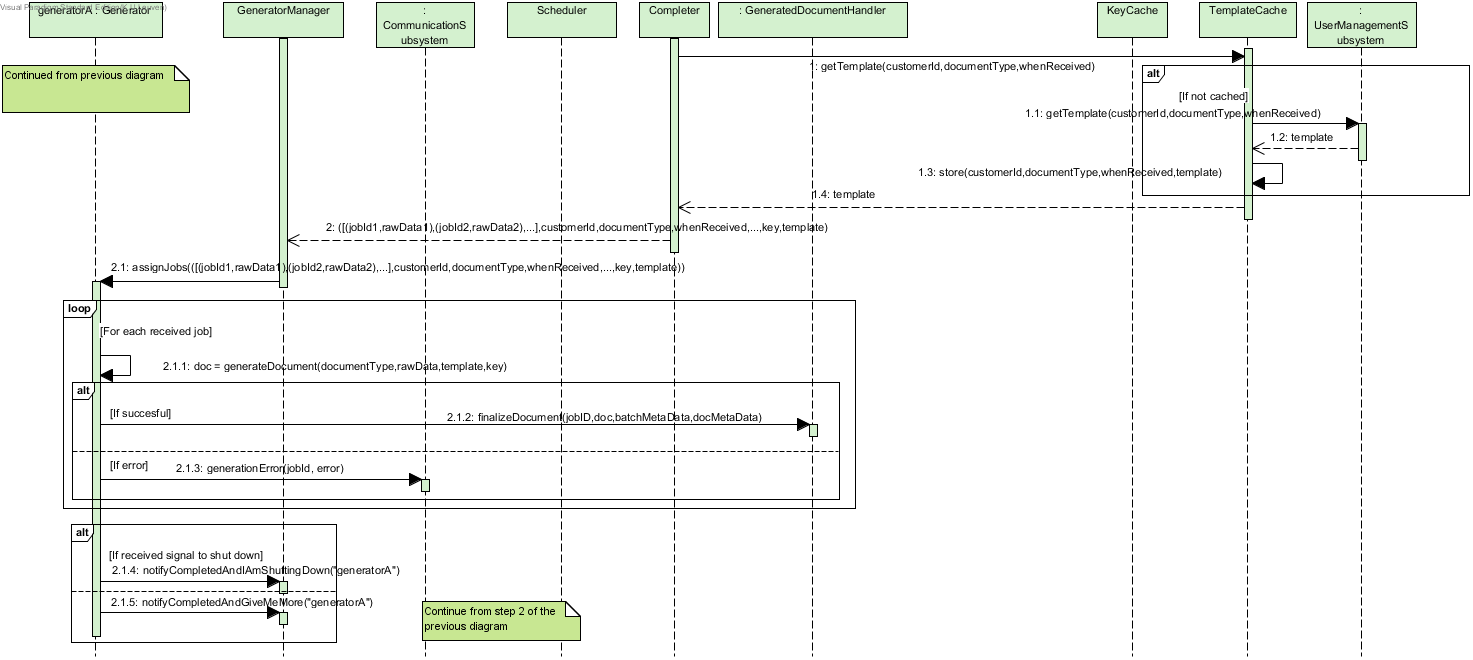
\includegraphics[width=\textwidth]{figures/UC4_5 - ProcessJobs2.png}
    %\missingfigure[figwidth=0.8\textwidth]{Sequence diagram scenario 1}
    \caption{Continuation of system behavior for Use Cases 4 and 5.
        }\label{fig:seq_uc45_2}
\end{figure}

\subsection{UC6 - Deliver document via e-mail}
Shortly describe the scenario shown in this subsection.
Show the complete scenario using one or more sequence diagrams.

\begin{figure}[!htp]
    \centering
    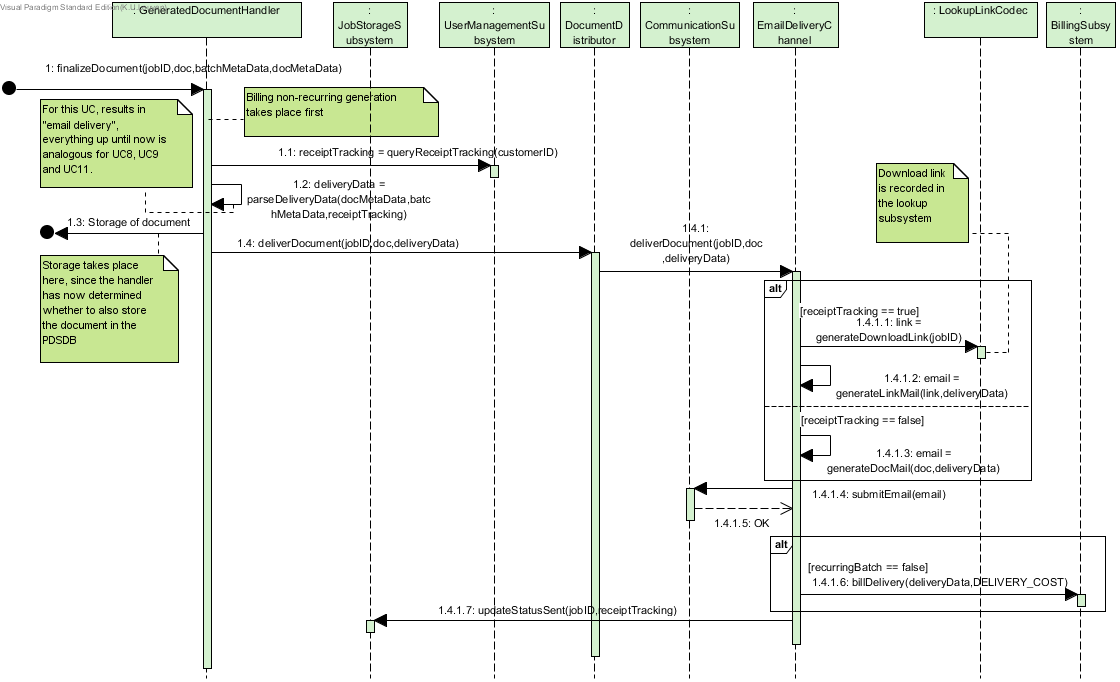
\includegraphics[width=\textwidth]{figures/UC6 - Deliver document via e-mail.png}
    %\missingfigure[figwidth=0.8\textwidth]{Sequence diagram scenario 1}
    \caption{The system behavior for the first scenario.
        }\label{fig:seq_uc6}
\end{figure}

\subsection{UC7 - Signal e-mail delivery failure}
Shortly describe the scenario shown in this subsection.
Show the complete scenario using one or more sequence diagrams.

\begin{figure}[!htp]
    \centering
    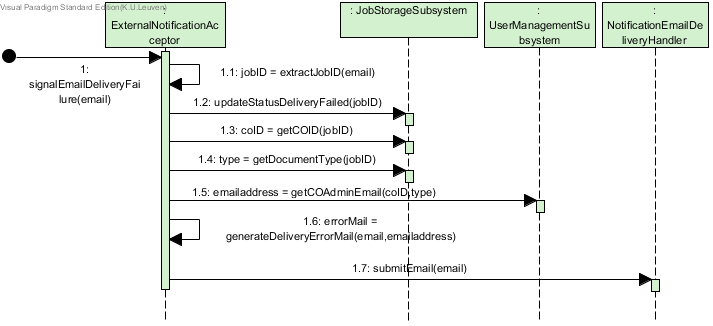
\includegraphics[width=\textwidth]{figures/UC7 - Signal e-mail delivery failure.png}
    %\missingfigure[figwidth=0.8\textwidth]{Sequence diagram scenario 1}
    \caption{The system behavior for the first scenario.
        }\label{fig:seq_uc7}
\end{figure}

\subsection{UC10 - Zoomit Receipt Confirmation}
Shortly describe the scenario shown in this subsection.
Show the complete scenario using one or more sequence diagrams.

\begin{figure}[!htp]
    \centering
    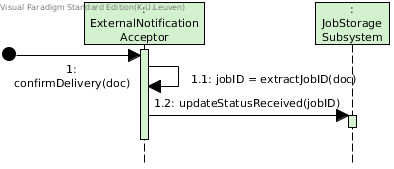
\includegraphics[width=\textwidth]{figures/UC10 - Zoomit Receipt Confirmation.png}
    %\missingfigure[figwidth=0.8\textwidth]{Sequence diagram scenario 1}
    \caption{The system behavior for the first scenario.
        }\label{fig:seq_uc10}
\end{figure}

\subsection{UC11a - Storing a document in the PDS}
Shortly describe the scenario shown in this subsection.
Show the complete scenario using one or more sequence diagrams.

\begin{figure}[!htp]
    \centering
    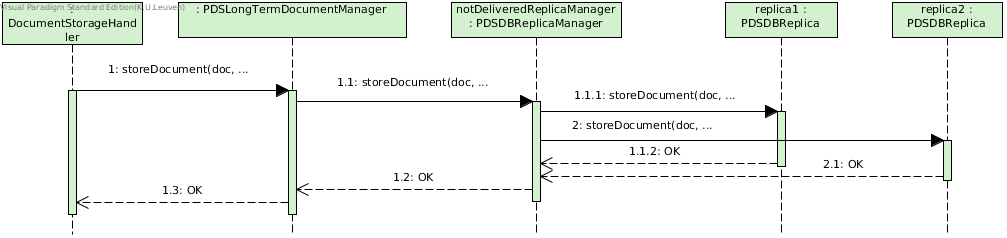
\includegraphics[width=\textwidth]{figures/UC11a - Storing a document in the PDS.png}
    %\missingfigure[figwidth=0.8\textwidth]{Sequence diagram scenario 1}
    \caption{The system behavior for the first scenario.
        }\label{fig:seq_uc11a}
\end{figure}

\subsection{UC14 - Consult document in PDS}
Shortly describe the scenario shown in this subsection.
Show the complete scenario using one or more sequence diagrams.

\begin{figure}[!htp]
    \centering
    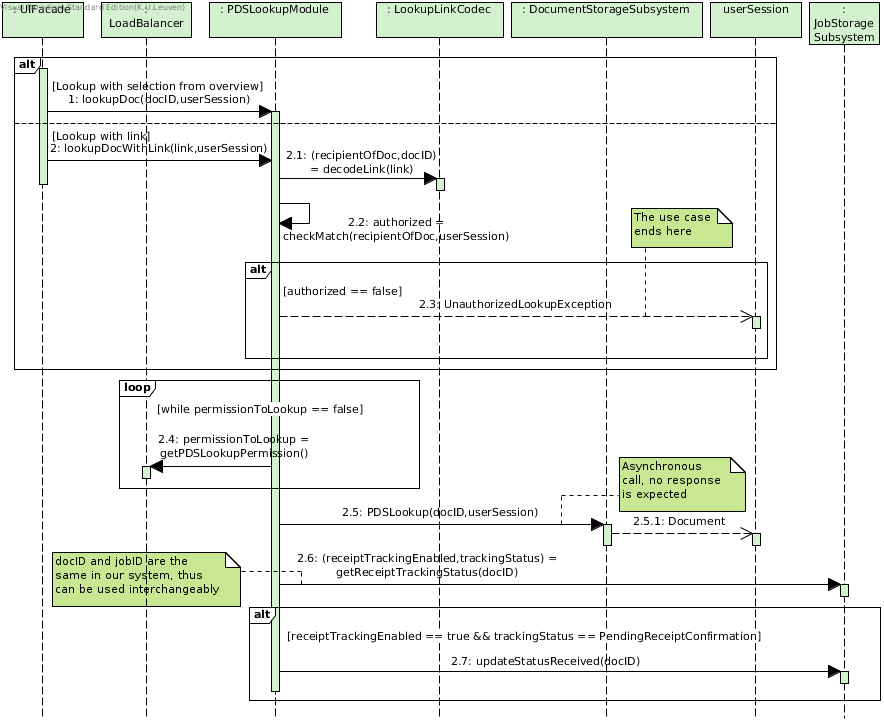
\includegraphics[width=\textwidth]{figures/UC14 - Consult document in PDS.png}
    %\missingfigure[figwidth=0.8\textwidth]{Sequence diagram scenario 1}
    \caption{The system behavior for the first scenario.
        }\label{fig:seq_uc14}
\end{figure}

\subsection{UC15 - Download document via unique link}
Shortly describe the scenario shown in this subsection.
Show the complete scenario using one or more sequence diagrams.

\begin{figure}[!htp]
    \centering
    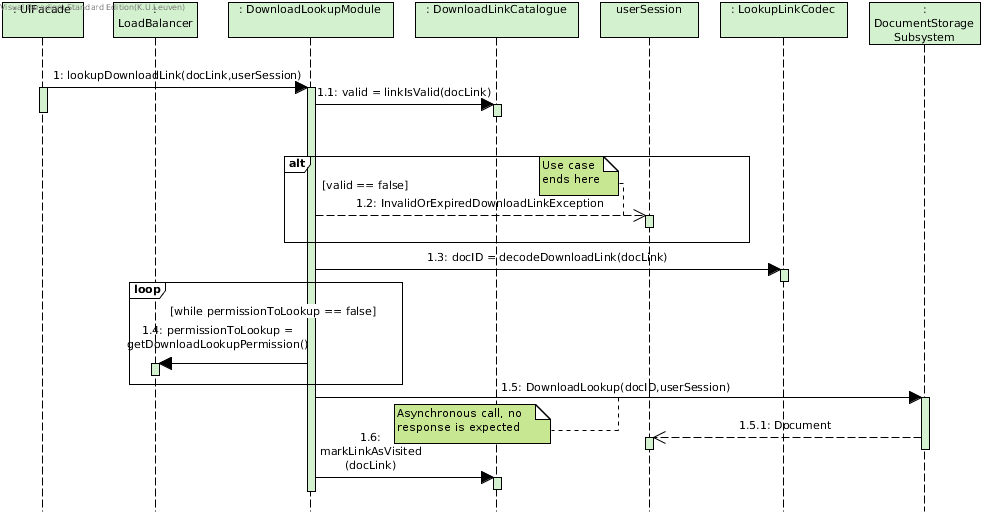
\includegraphics[width=\textwidth]{figures/UC15 - Download document via unique link.png}
    %\missingfigure[figwidth=0.8\textwidth]{Sequence diagram scenario 1}
    \caption{The system behavior for the first scenario.
        }\label{fig:seq_uc15}
\end{figure}

\subsection{UC17 - Register to PDS}
Shortly describe the scenario shown in this subsection.
Show the complete scenario using one or more sequence diagrams.

\begin{figure}[!htp]
    \centering
    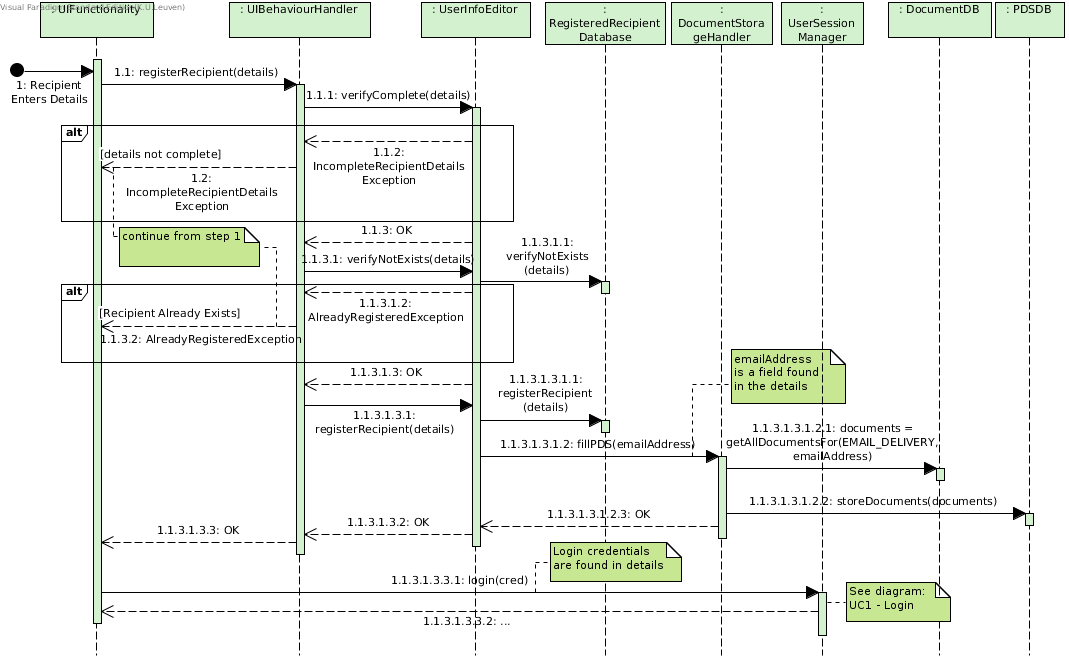
\includegraphics[width=\textwidth]{figures/UC17 - Register to PDS.png}
    %\missingfigure[figwidth=0.8\textwidth]{Sequence diagram scenario 1}
    \caption{The system behavior for the first scenario.
        }\label{fig:seq_uc17}
\end{figure}

\subsection{UC21 - Consult Status of all Document Processing Jobs}
Shortly describe the scenario shown in this subsection.
Show the complete scenario using one or more sequence diagrams.

\begin{figure}[!htp]
    \centering
    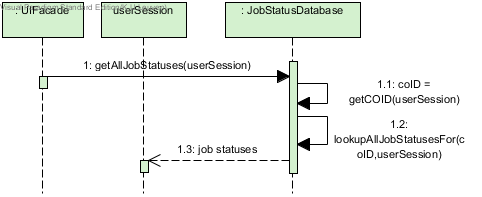
\includegraphics[width=\textwidth]{figures/UC21 - Consult Status of all Document Processing Jobs.png}
    %\missingfigure[figwidth=0.8\textwidth]{Sequence diagram scenario 1}
    \caption{The system behavior for the first scenario.
        }\label{fig:seq_uc21}
\end{figure}

\subsection{UC22 - Notify CO administrator}
Shortly describe the scenario shown in this subsection.
Show the complete scenario using one or more sequence diagrams.

\begin{figure}[!htp]
    \centering
    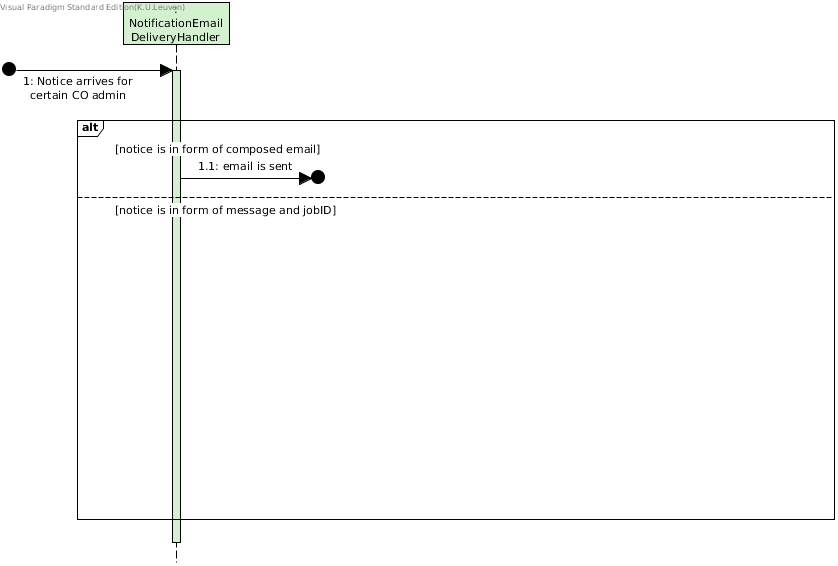
\includegraphics[width=\textwidth]{figures/UC22 - Notify CO administrator.png}
    %\missingfigure[figwidth=0.8\textwidth]{Sequence diagram scenario 1}
    \caption{The system behavior for the first scenario.
        }\label{fig:seq_uc22}
\end{figure}